\documentclass[tp]{lcc}

% add latex preamble
% para la bibliografía se requiere biber y configurar texstudio

% Latex packages
\usepackage[utf8]{inputenc}
\usepackage[T1]{fontenc} % para copiar acentos en español del pdf y permite acentos en las notas
\usepackage[spanish]{babel}
\usepackage[per-mode = symbol]{siunitx} % para manejar las unidades
\usepackage{multimedia} % to add videos with \movie command
\usepackage{multirow}
\usepackage{graphicx}
\usepackage{xcolor}
\usepackage{amsmath} % bmatrix
\usepackage[makeroom]{cancel} % \cancel to cancel terms in math equations
\renewcommand{\CancelColor}{\color{red}} % set red color for \cancel command
\usepackage[caption=false]{subfig} % caption = false elimina la palabra "Figura" del caption
\usepackage{import} % para el comando import (se usa para pdf_tex)
\captionsetup[subfigure]{labelformat=empty} % remover el indice del caption de la subfigura
\usepackage{booktabs} % \toprule \midrule \bottomrule
\usepackage[backend=biber]{biblatex} % set biber to format references. Must configure Biber in Texstudio
\usepackage{csquotes} % to remove warning triggered by biblatex and babel
\usepackage{algorithm} % to put captions to the algorithmics environmets
\usepackage{algpseudocode} % to write algorithm
\usepackage{tikz} % to use tikz
\usetikzlibrary{fit} % to fit a node around other nodes in tikz
\usepackage[export]{adjustbox} % valign in subfloat
\usepackage{colortbl} % to paint cells in a table

% Color commands for annotations
\newcommand\TODO[1]{\textbf{\textcolor{red}{#1}}} %  TODO notes

% Graphic paths
\graphicspath{{./images/}}

% listings configuration for C code
\usepackage{listings} % code
\definecolor{commentgreen}{RGB}{2,112,10}
\definecolor{eminence}{RGB}{108,48,130}
\definecolor{weborange}{RGB}{255,165,0}
\definecolor{frenchplum}{RGB}{129,20,83}

\lstset{ % spanish characters for listings package
	inputencoding=latin1,
    columns=fullflexible,
	breaklines=true,
	tabsize=2,
	showstringspaces=false,
	basicstyle=\ttfamily,
	backgroundcolor=\color{lightgray}, % Choose background color
	literate={á}{{\'a}}1
	{ã}{{\~a}}1
	{é}{{\'e}}1
	{ó}{{\'o}}1
	{í}{{\'i}}1
	{ñ}{{\~n}}1
	{¡}{{!`}}1
	{¿}{{?`}}1
	{ú}{{\'u}}1
	{Í}{{\'I}}1
	{Ó}{{\'O}}1
    {-}{-}1
}

\lstdefinestyle{cpp}{ % spanish characters for listings package
    language=C++,
   	commentstyle=\color{commentgreen},
    keywordstyle=\color{eminence},
    stringstyle=\color{red},
    emph={int,char,double,float,unsigned,void,bool},
    emphstyle={\color{blue}}
}

\lstdefinestyle{bash}{ % spanish characters for listings package
	language=Bash
}

\lstdefinestyle{xml}{
	language=XML,
	morekeywords={encoding,xs:schema,xs:element,xs:complexType,xs:sequence,xs:attribute}
}

\lstdefinestyle{cmake}{
	language=make, % there is no cmake support in listings
}

\lstdefinestyle{python}{
    language=python,
}


%%%%% PARA QUE EN LAS TABLAS SE PUEDA PONER UN SALTO DE LINEA DENTRO DE UNA CELDA
\newcommand{\specialcell}[2][c]{%
    \begin{tiny}
        \begin{tabular}[#1]{@{}c@{}}#2\end{tabular}  
    \end{tiny}
}
%%%%%%%%%%%%%%%%%%%%%%%%%%%%%%%%%%%%%%%%%%%%%%%%%%%%%%%%%%%%%%%%%%%%%%%%

%%%%% PARA QUE LAS TABLAS TENGAN TODAS LAS COLUMNAS CENTRADAS Y DE IGUAL TAMAÑO
\usepackage{tabularx}
\renewcommand{\tabularxcolumn}[1]{>{\centering\arraybackslash}m{#1}}
%%%%%%%%%%%%%%%%%%%%%%%%%%%%%%%%%%%%%%%%%%%%%%%%%%%%%%%%%%%%%%%%%%%%%%%%



% add math preamble
\usepackage{amsmath}
\usepackage{amssymb}
\usepackage{amsopn}
\usepackage{mathtools}

% math
\renewcommand{\vec}[1]{\boldsymbol{\mathbf{#1}}}
\newcommand{\norm}[1]{\lVert#1\rVert}

% Declare arg max and arg min functionss
\DeclareMathOperator*{\argmax}{arg\,max}
\DeclareMathOperator*{\argmin}{arg\,min}

% Homogeneous decoration function
\newcommand{\homo}[1]{\dot{#1}}


% Declare projection as math function
\DeclareMathOperator{\proj}{proj}
\newcommand{\fromCoord}[2]{{#1}_\mathrm{#2}}
\newcommand{\toCoord}[2]{\prescript{\mathrm{#2}}{}{#1}}
\newcommand{\worldCoordSystem}{\mathrm{w}}
\newcommand{\bodyCoordSystem}{\mathrm{B}}
\newcommand{\cameraCoordSystem}{\mathrm{c}}
\newcommand{\point}{\vec{p}}
\newcommand{\worldPoint}{\toCoord{\point}{\worldCoordSystem}}
\newcommand{\imagePoint}{\vec{u}}
\newcommand{\cameraPoint}{\toCoord{\point}{\cameraCoordSystem}}
\newcommand{\homoWorldPoint}{\toCoord{\homo{\point}}{\worldCoordSystem}}
\newcommand{\homoImagePoint}{\homo{\imagePoint}}
\newcommand{\homoCameraPoint}{\toCoord{\homo{\point}}{\cameraCoordSystem}}
\newcommand{\measurement}{\vec{z}}
\newcommand{\prediction}{\hat{\vec{z}}}
\newcommand{\seMatrix}{\vec{\xi}}
\newcommand{\transform}[2]{\toCoord{\fromCoord{\seMatrix}{#2}}{#1}}
\newcommand{\pointCoord}[1]{\toCoord{\point}{#1}}
\newcommand{\rotation}{\vec{R}}
\newcommand{\rotationCoord}[2]{\toCoord{\fromCoord{\rotation}{#2}}{#1}}
\newcommand{\translation}{\vec{t}}
\newcommand{\translationCoord}[2]{\toCoord{\fromCoord{\translation}{#2}}{#1}}
\newcommand{\intrinsicMatrix}{\vec{K}}
\newcommand{\principalPoint}{\vec{c}}
\newcommand{\reprojectionError}{u}
\newcommand{\projectionMatrix}{\vec{P}}
\newcommand{\cameraCenter}{\vec{o}}
\newcommand{\essentialMatrix}{\vec{E}}
\newcommand{\inverse}[1]{{#1}^{-1}}

% Motion model
\newcommand{\position}{\vec{p}}
\newcommand{\orientationQuaternion}{\vec{q}}
\newcommand{\predictedPosition}{\hat{\vec{p}}}
\newcommand{\predictedOrientationQuaternion}{\hat{\vec{q}}}
\newcommand{\linearVelocity}{\vec{v}}
\newcommand{\angularVelocity}{\vec{\omega}}

\DeclareMathOperator{\slerpOp}{slerp}
\newcommand{\slerp}[1]{\slerpOp{\left( #1 \right)}}

% Map structure
\newcommand{\map}{M}
\newcommand{\keyframesSet}{K}
\newcommand{\mapPointsSet}{P}
\newcommand{\observedMapPoints}{O}
\newcommand{\covisibilityKeyframes}{CK}
\newcommand{\localMap}{local\_map}



% Bundle Adjutment
\newcommand{\update}{\vec{\delta}}
\newcommand{\incremental}{\hat{\update}}


% Loop Closure names

% scaled operators and letters to fancy view
\newcommand{\sminus}{\scalebox{0.5}[1.0]{$-$}}
\newcommand{\splus}{\scalebox{0.6}[0.6]{$+$}}
\newcommand{\curr}{c}
\newcommand{\sind}[1]{\scalebox{0.6}[0.6]{$#1$}}
\newcommand{\ind}[1]{\scalebox{0.7}[0.7]{$#1$}}

\newcommand{\keyframe}{\vec{K}}
\newcommand{\bowVector}{\vec{v}}
\newcommand{\lcError}{\vec{\Omega}}
\newcommand{\relativeTransformation}{\seMatrix}
\DeclareMathOperator{\interpolate}{interpolate}

\newcommand{\relativeMotion}{\vec{\delta}}
\newcommand{\groundTruth}[1]{{#1}^{*}}



% definición del operador rot()
\DeclareMathOperator{\rotationOp}{rot}
\newcommand{\getRotation}[1]{\rotationOp{\left( #1 \right)}}

\DeclareMathOperator{\translationOp}{trans}
\newcommand{\getTranslation}[1]{\translationOp{\left( #1 \right)}}









\codigo{R-521}
\materia{Robótica Móvil}
\titulo{Graph SLAM}

% Mostrar soluciones
%\soluciones
%\commentstrue


\usepackage{biblatex}
%\addbibresource{refs.bib}

\begin{document}
\maketitle


\section*{Disclaimer}
This homework is based on the Homework 7 -- SLAM of the NA 568 Mobile Robotics: Methods \& Algorithms -- Winter 2022 created by Maani Ghaffari -- University of Michigan
%\title{NA 568 Mobile Robotics: Methods \& Algorithms \\ Winter 2022 -- Homework 7 -- SLAM}
%\author{Maani Ghaffari \\ University of Michigan}
%\date{March 19, 2022}

\section*{Submission Instructions}

\begin{enumerate}
    \item A .tar.gz or .zip file containing a directory named after your uniqname with the structure shown below. \\
    \lstinline[style=bash]{alincoln_hw7.zip:} \\
    \lstinline[style=bash]{alincoln_hw7/} \\
    \lstinline[style=bash]{alincoln_hw7/YOUR_WORKING_CODE} \\
    You may use C++, Python, or MATLAB for your programming.

    \item A PDF with the written portion of your write-up. Scanned versions of hand-written documents, converted to PDFs, are perfectly acceptable. No other formats (e.g., doc) are acceptable. Your PDF file should adhere to the following naming convention: \lstinline[style=bash]{alincoln_hw7.pdf}.

    \item Submit your complete source code. We will compile and run your code for evaluation.
\end{enumerate}

\section*{Pose Graph SLAM using GTSAM Library}
In this homework, you’re going to solve the pose graph SLAM problem using the GTSAM library. If you are not familiar with GTSAM, a detailed tutorial is on their website: \url{https://gtsam.org/tutorials/intro.html}. To install GTSAM in c++, you’ll have to clone the code from the repository: \url{https://github.com/borglab/gtsam}, checkout (using git) the latest version and build the library following the instruction.

After you successfully install GTSAM, write a function to read G2O \footnote{\url{https://github.com/RainerKuemmerle/g2o/wiki/File-Format}} files and solve the graph optimization problem for both 2D and 3D cases using GTSAM. In this assignment, we use datasets provided at \url{https://lucacarlone.mit.edu/datasets/}.

While GTSAM is developed using C++, it also provides both MATLAB and Python wrapper. In this assignment, you’re free to use any of those languages.

\subsection*{GTSAM Installation Guide}
Below we provide an installation guide for GTSAM libraries, then we introduce C++, MATLAB, and python versions of them respectively.

\subsubsection*{GTSAM library}
The first step is to clone and install GTSAM library. Detailed instruction can be found in the repository.

\textbf{Remark 1.} \textit{If you are planning to use MATLAB or python wrapper, you may skip this part.}

\textbf{Remark 2.} \textit{GTSAM requires the Eigen library. It can be downloaded and installed from here: \url{http://eigen.tuxfamily.org/index.php?title=Main_Page}}

\textbf{Remark 3.} \textit{Please notice prerequisites: Boost >= 1.58 (Ubuntu: sudo apt-get install libboost-all-dev); CMake >= 3.0 (Ubuntu: sudo apt-get install cmake); A modern compiler, i.e., at least gcc 4.7.3 on Linux.}

\begin{itemize}
    \item Go to gtsam repository \url{https://github.com/borglab/gtsam} and click the green clone or download button on the right hand side to clone the repository to your machine.
    \item In the terminal, enter command (this will allow you to navigate to the repository)
    
    \lstinline[style=bash]{cd <path_to_your_repository>}
    
    \item Then create a new folder named build by
    
    \lstinline[style=bash]{mkdir build}
    
    \item Navigate into the build folder
    
    \lstinline[style=bash]{cd build}
    
    \item run cmake to create essential links for building files (\textbf{Note}: if you want to use the python wrapper, you will have to do something different here. Please jump to the python wrapper section)
    
    \lstinline[style=bash]{cmake ..}
\end{itemize}

\textbf{Remark 4.} \textit{If you have error saying could not find Boost, you may try manually install boost following \href{https://www.boost.org/doc/libs/1_66_0/more/getting_started/unix-variants.html\#get-boost}{this tutorial} and make sure you are pointing to the correct directory by adding following commands in CMakeList.txt :}



\begin{lstlisting}[style=bash]
SET (BOOST_ROOT "<your_boost_path>")
SET (BOOST_INCLUDEDIR "<your_boost_path>/boost")
SET (BOOST_LIBRARYDIR "<your_boost_path>/libs")
SET (BOOST_MIN_VERSION "1.58.0")
set (Boost_NO_BOOST_CHAKE ON)
\end{lstlisting}

\begin{itemize}
    \item make the file to the build folder (The command -j10 indicates the number of threads to be used during make. It'll make the compilation faster. I recommend using your max number of cores - 2, otherwise your machine may get stuck. I have 12 threads on my machine, so I use -j10.) \lstinline[style=bash]{make -j10}
    \item install the gtsam library to your machine. \lstinline[style=bash]{sudo make install -j10}
    \item At this step, you will be able to see the path where all the packages are installing to. If later you somehow cannot link the install path to your code, you can come back to this step and see where it is installed to.
\end{itemize}

\subsubsection*{C++}
If you want to use C++, you don't have to install anything else. All you need to do is to find and link GTSAM library by adding the below context to your CMakeList.txt file.

\begin{lstlisting}[style=cmake]
find_package(GTSAM_REQUIRED)
include_directories(${GTSAM_INCLUDE_DIR})
target_link_libraries(<your_project> <your_project_lib> gtsam)
\end{lstlisting}

You may refer to some c++ gtsam examples \url{https://github.com/borglab/gtsam/tree/develop/examples}.

\subsubsection*{MATLAB Wrapper}
If you have a newer Ubuntu system (later than 10.04), you must make a small modification to your MATLAB installation, due to MATLAB being distributed with an old version of the C++ standard library. Delete or rename all files starting with libstdc++ in your MATLAB installation directory, in paths:

\begin{itemize}
    \item \lstinline[style=bash]|/usr/local/MATLAB/{version}/sys/os/{system}|
    \item \lstinline[style=bash]|/usr/local/MATLAB/{version}/bin/{system}|
\end{itemize}

For MATLAB wrapper, you can do it in two ways:

\begin{enumerate}
    \item download the precompiled wrapper from \url{http://www.borg.cc.gatech.edu/download.html},
    \item or install from sources following the instructions in \url{https://github.com/borglab/gtsam/tree/develop/matlab}.
\end{enumerate}

We recommend using the pre-compiled wrapper if you are not familiar with linux systems. Below are instructions on how to add the pre-compiled MATLAB wrapper to your toolbox.

\begin{itemize}
    \item Download the pre-compiled wrapper here. Download precompiled MATLAB toolbox (Works with MATLAB R2011a and later) depends on your system OS (Mac OS 64-bit / Linux 64-bit / Windows 64-bit).
    \item Extract the folder. (\textbf{Note: for linux system}, after extracting, you'll have to right click on the extracted file $\rightarrow$ Open With $\rightarrow$ Archive Mounter. Your will then see a \lstinline[style=bash]{gtsam-toolbox-3.2.0-lin64} on your left side along with Computer, OS... The folder inside named \lstinline[style=bash]{gtsam_toolbox} is the folder we want to use.)
    \item Put the \lstinline[style=bash]{gtsam_toolbox} folder under \lstinline[style=bash]{<YOUR_MATLAB_INSTALL_PATH>/toolbox/}
    \item Every time you open your MATLAB, at the left side of your GUI, navigate to your \lstinline[style=bash]{gtsam_toolbox} $\rightarrow$ right click $\rightarrow$ add to path $\rightarrow$ selected folder. Then you should be able to run the example codes under the example folder. Or you can add the following commends as your first part of code.
    \begin{lstlisting}[style=bash]
addpath('<your_gtsam_toolbox_path>')
import gtsam.*
    \end{lstlisting}
\end{itemize}

You may refer to some matlab gtsam examples in \lstinline[style=bash]{gtsam_toolbox/gtsam_examples} folder.

\subsubsection*{Python Wrapper}

Download and Install Anaconda from \url{https://www.anaconda.com/download}

\begin{lstlisting}[style=bash] 
conda create -n gtsam_env python=<your_python_version>
conda activate gtsam_env
conda install -c conda-forge cmake eigen pybind11 boost numpy matplotlib python-graphviz conda-forge::plotly conda-forge::pandas conda-forge::nbformat
\end{lstlisting}

\begin{lstlisting}[style=bash] 
git clone https://github.com/borglab/gtsam.git
cd gtsam
mkdir build && cd build
conda install -r <gtsam_folder>/python/requirements.txt
cmake .. -DGTSAM_BUILD_PYTHON=1 -DGTSAM_PYTHON_VERSION=<your_python_version>
make -j2 (2 is the number of threads you want to use)
make python-install
\end{lstlisting}

You may refer to some python gtsam examples in \url{https://github.com/borglab/gtsam/tree/develop/python/gtsam/examples}.

\section{2D Graph SLAM}
\subsection{A.}
Write a function to read 2D Intel dataset\footnote{\url{https://www.dropbox.com/s/vcz8cag7bo0zlaj/input_INTEL_g2o.g2o?dl=0}} from G2O format and output poses and edges. These poses and edges are used in later problems. It can be any form you like as long as you can use it to generate the correct result.

For 2D data, the pose in G2O format is \lstinline[style=bash]{[VERTEX_SE2 i x y theta]} and the edge in G2O format is \lstinline[style=bash]{[EDGE_SE2 i j x y theta info(x, y, theta)]}, where \lstinline[style=bash]{info(x, y, theta)} is a $1 \times 6$ vector \lstinline[style=bash]{[q11 q12 q13 q22 q23 q33]} where the elements are the upper-triangle matrix of the $3 \times 3$ information matrix:

\begin{equation*}
    \Omega = \begin{bmatrix} q_{11} & q_{12} & q_{13} \\ q_{12} & q_{22} & q_{23} \\ q_{13} & q_{23} & q_{33} \end{bmatrix}.
\end{equation*}

By inverting this information matrix, you can obtain the covariance matrix for the noise model.

You may look into detail in the g2o repository\footnote{\url{https://github.com/RainerKuemmerle/g2o/wiki/File-Format-SLAM-2D}}.

\textbf{Remark 5.} \textit{If you use \lstinline[style=bash]{readG2o()} and \lstinline[style=bash]{load2D()} functions provided by GTSAM, then you will not be able to solve the graph incrementally (task~\ref{sec:incremental_solution} in this homework).}

\textbf{Hint:} You may use \lstinline[style=bash]{fscanf()}, \lstinline[style=bash]{textscan()}, or \lstinline[style=bash]{readcell()} functions with proper formatSpec from MATLAB and check if the first element in the input is \lstinline[style=bash]{VERTEX_SE2} or \lstinline[style=bash]{EDGE_SE2}.

\subsection{B. Batch Solution}
A batch solution means when we construct the entire graph and solve it at the end altogether. Load \lstinline[style=bash]{data/input_INTEL_g2o.g2o} and construct a 2D nonlinear factor graph using GTSAM. Use the Gauss-Newton solver. Visualize and compare the optimized trajectory against the initial trajectory. Include the plot in your pdf. Describe the graph construction process and its parameters.

\textbf{Remark 6.} \textit{For this problem, Gauss Newton solver will fall into a local minimum if we don't give any perturbation. It is okay to submit a plot that doesn't work as expected, but please include discussions about why is this happening.}

\textbf{Hint:} You may use \lstinline[style=bash]{NonLinearFactorGraph} as your graph, use \lstinline[style=bash]{GaussNewtonOptimizer} as you optimizer, use \lstinline[style=bash]{Values} for your initial estimation, \lstinline[style=bash]{noiseModel.Gaussian.Covariance()} for your noise model, \lstinline[style=bash]{graph.add()} and \lstinline[style=bash]{initial.insert()} functions as you see fit. However, function names might be different for different versions of gtsam.

\subsection{C. Incremental Solution}
\label{sec:incremental_solution}
Use ISAM2 solver to optimize the trajectory incrementally (as you build the graph gradually). A detailed algorithms is described in Algorithm~\ref{alg:isam2}. Visualize and compare the optimized trajectory against the initial trajectory. Include the plot in your pdf. Describe the graph construction process and its parameters.

\begin{algorithm}
    \caption{\lstinline[style=bash]{incremental_solution_2d(poses, edges)}}
    \label{alg:isam2}
    \begin{algorithmic}[1]    
    \Require poses: a N x 4 array that each row is $pose=(id_{p},x,y,\theta)$; edges: a M x 11 array that each row is $edge=(id_{e1},id_{e2},dx,dy,d\theta,info)$
    \State $isam \leftarrow$ gtsam.ISAM2() \Comment{Initialize isam solver}
    \For{every pose in poses}
        \State $graph \leftarrow$ NonlinearFactorGraph \Comment{Initialize the factor graph}
        \State $initialEstimate \leftarrow$ Values \Comment{Initialize the initial estimation}
        \State $(id_{p},x,y,\theta) \gets pose$ \Comment{Extract information from the current pose}
        \If{$id_{p} == 0$}
            \State $priorNoise \leftarrow$ some noiseModel \Comment{Use a predefined noise model}
            \State $graph.add(PriorFactorPose2(0,Pose2(x,y,\theta),priorNoise))$
            \State $initialEstimate.insert(id_{p},\text{Pose2}(x,y,\theta))$
        \Else \Comment{Not the first pose}
            \State $prevPose \gets result.at(id_{p}-1)$ \Comment{Use last optimized pose}
            \State $initialEstimate.insert(id_{p},prevPose)$
        \EndIf
        \For{every edge in edges}
            \State $(id_{e1},id_{e2},dx,dy,d\theta,info) \gets edge$ \Comment{Extract information from the current edge}
            \If{$id_{e2} == id_{p}$}
                \State $cov=construct\_covariance(info)$ \Comment{Construct a covariance matrix from the information vector.}
                \State $Model \leftarrow$ noiseModel.Gaussian.Covariance($cov$)
                \State $graph.add(BetweenFactorPose2(id_{e1},id_{e2},\text{Pose2}(dx,dy,d\theta),Model)$
            \EndIf
        \EndFor
        \State $isam.update(graph,initialEstimate)$
        \State $result=isam.calculateEstimate$
    \EndFor
    \end{algorithmic}
\end{algorithm}

\textbf{Hint:} You may use \lstinline[style=bash]{NonLinearFactorGraph} as your graph, use \lstinline[style=bash]{gtsam.ISAM2()} as your update algorithm, use \lstinline[style=bash]{Values} for your initial estimation, and use \lstinline[style=bash]{graph.add()}, \lstinline[style=bash]{initial.insert()}, \lstinline[style=bash]{isam.update()}, and \lstinline[style=bash]{isam.calculateEstimate()} functions as you see fit. However, function names might be different for different versions of gtsam.

\section{3D Graph SLAM}
\subsection{A.}
Write a function to read 3D Garage G2O file\footnote{\url{https://www.dropbox.com/s/zu23p8d522qccor/parking-garage.g2o?dl=0}} from G2O format and output poses and edges.

For 3D data, the pose in G2O format is \lstinline[style=bash]{[VERTEX_SE3:QUAT i x y z qx qy qz qw]} where \lstinline[style=bash]{(x,y,z)} represents the translation and \lstinline[style=bash]{(qx,qy,qz,qw)} the rotation as a quaternion. The edge in G2O format is \lstinline[style=bash]{[EDGE_SE3:QUAT i j x y z qx qy qz qw info(x, y, z, qx, qy, qz)]}, where \lstinline[style=bash]{info(x, y, z, qx, qy, qz)} is a $1 \times 21$ vector of the $6 \times 6$ information matrix. After similar process in task 1 A, you can obtain the covariance matrix. You may look into detail in the g2o repository\footnote{\url{https://github.com/RainerKuenmerle/g2o/wiki/File-Format-SLAM-3D}}.

\textbf{Remark 7.} \textit{Please notice that the quaternion in MATLAB is in the order of \lstinline[style=bash]{[qw qx qy qz]} and is different from the order in g2o files which is \lstinline[style=bash]{[qx qy qz qw]}. You may use \lstinline[style=bash]{quat2rotm()} function in matlab to construct a rotation matrix from quaternion or use \lstinline[style=bash]{quat2tform()} function in matlab to construct a transformation matrix.}

\subsection{B. Batch Solution}
Load \lstinline[style=bash]{data/parking-garage.g2o} and construct a 3D nonlinear factor graph using GTSAM. Use the Gauss-Newton solver. Visualize and compare the optimized trajectory against the initial trajectory. Include a 3D plot or two 2D plots in your pdf. Describe the graph construction process and its parameters.

\subsection{C. Incremental Solution}
Use ISAM2 solver to optimize the trajectory incrementally. Visualize and compare the optimized trajectory against the initial trajectory. Include a 3D plot or two 2D plots in your pdf. Describe the graph construction process and its parameters.

\begin{figure}[!htbp]
    \centering
    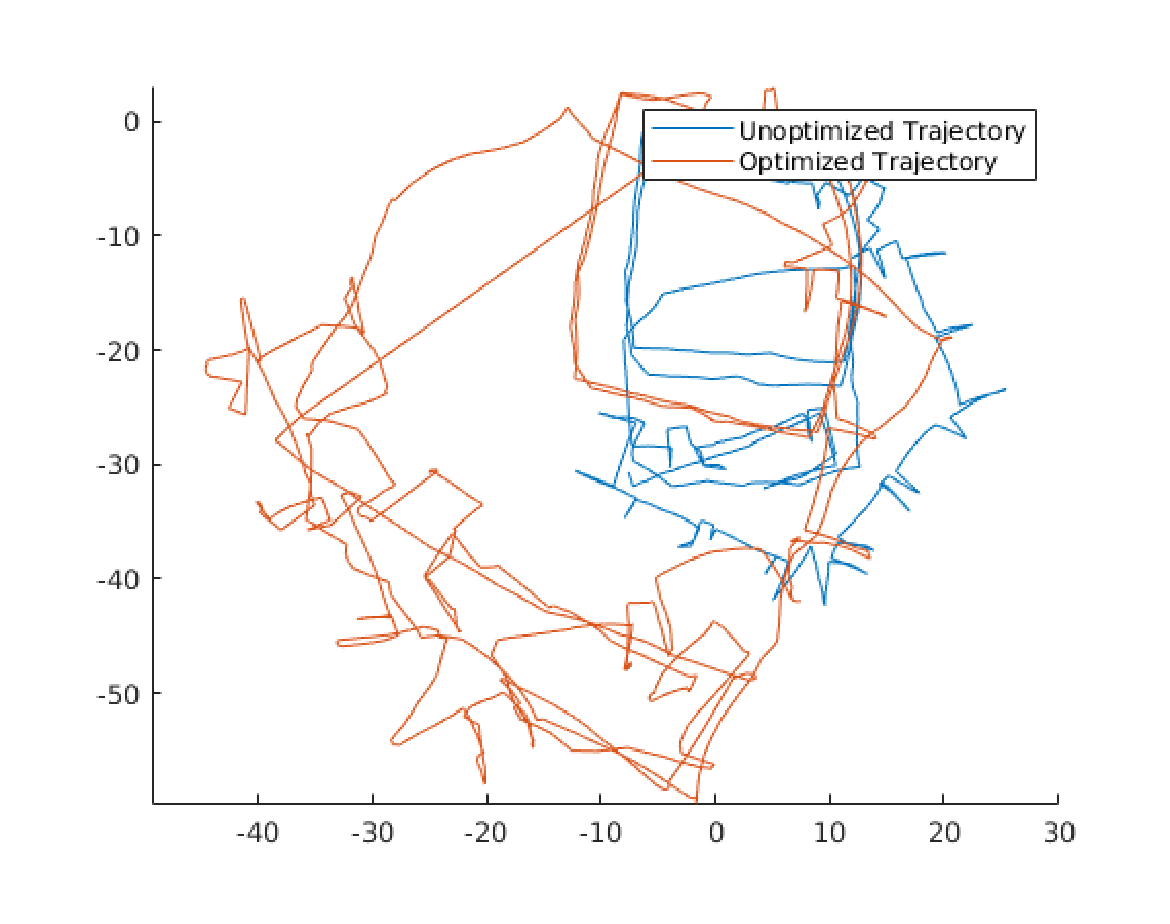
\includegraphics[width=0.6\textwidth]{images/result_task_1b.png}
    \caption{Expected result for task 1 B.}
    \label{fig:task1b}
\end{figure}

\begin{figure}[!htbp]
    \centering
    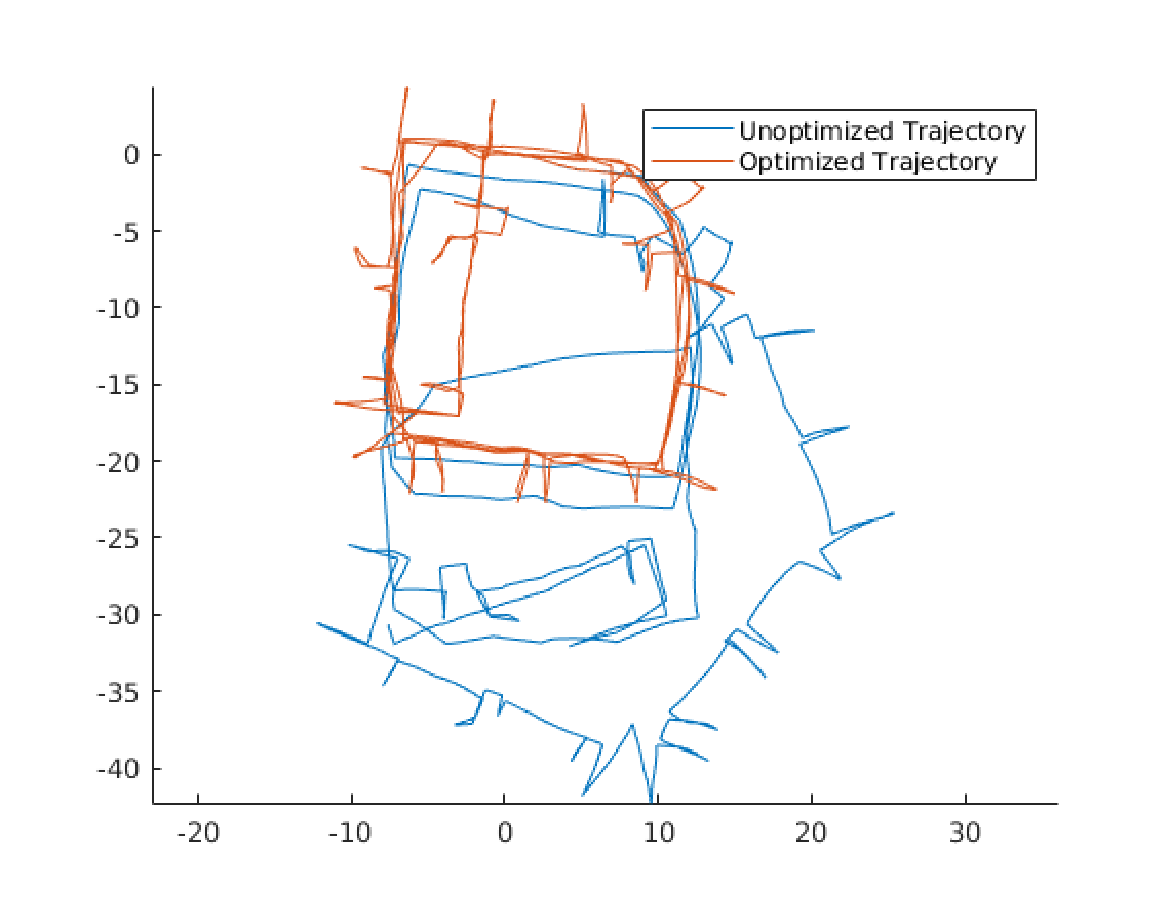
\includegraphics[width=0.7\textwidth]{result_task_1c.png}
    \caption{Expected result for task 1 C.}
    \label{fig:task1c}
\end{figure}

\begin{figure}[!htbp]
    \centering
    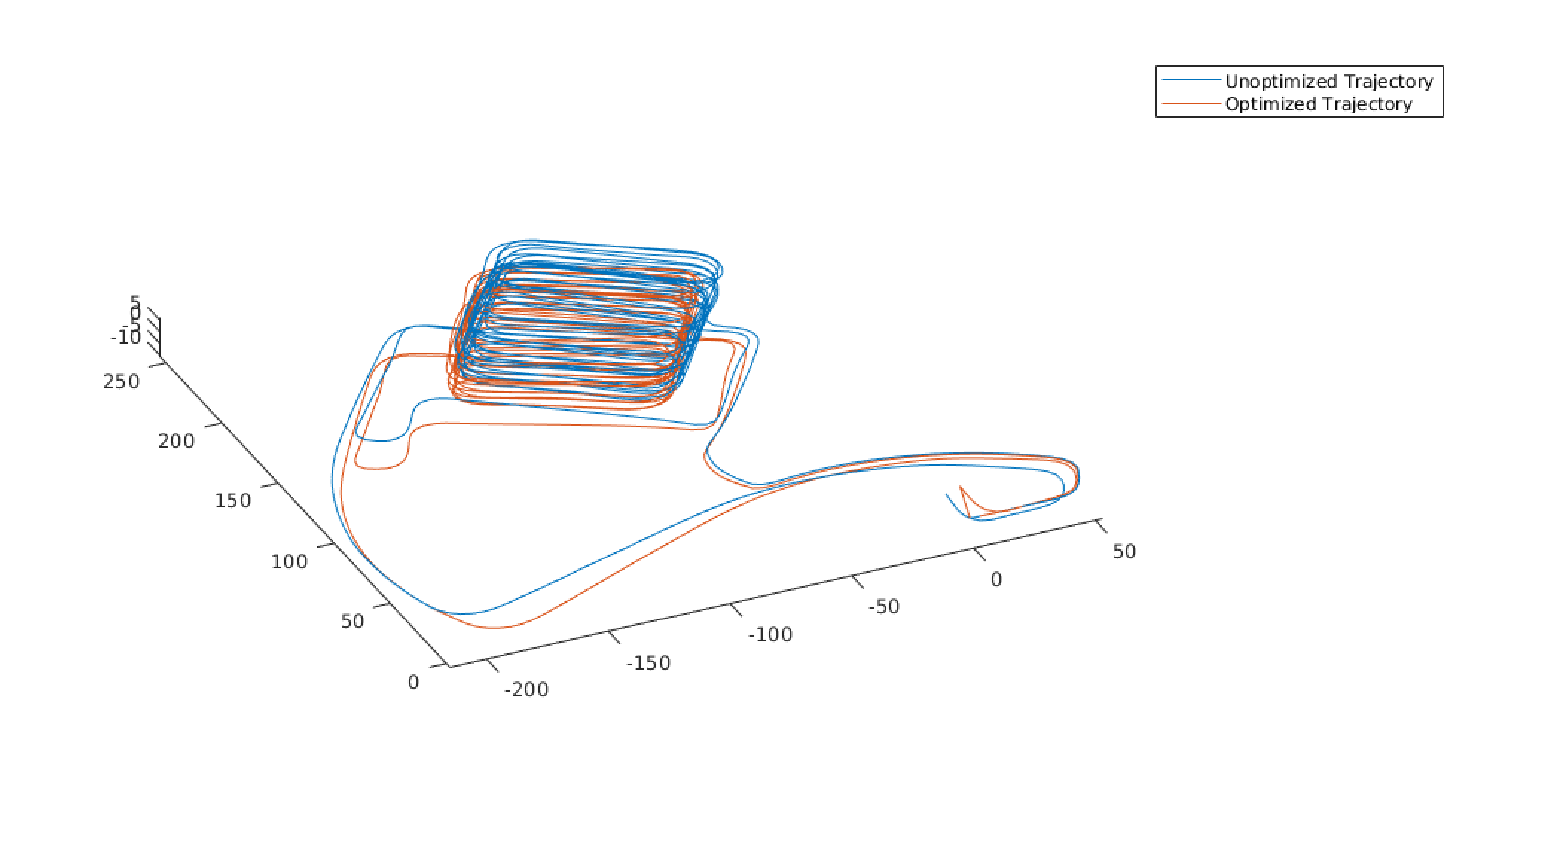
\includegraphics[width=0.8\textwidth]{result_task_2b.png}
    \caption{Expected result for task 2 B.}
    \label{fig:task2b}
\end{figure}

\begin{figure}[!htbp]
    \centering
    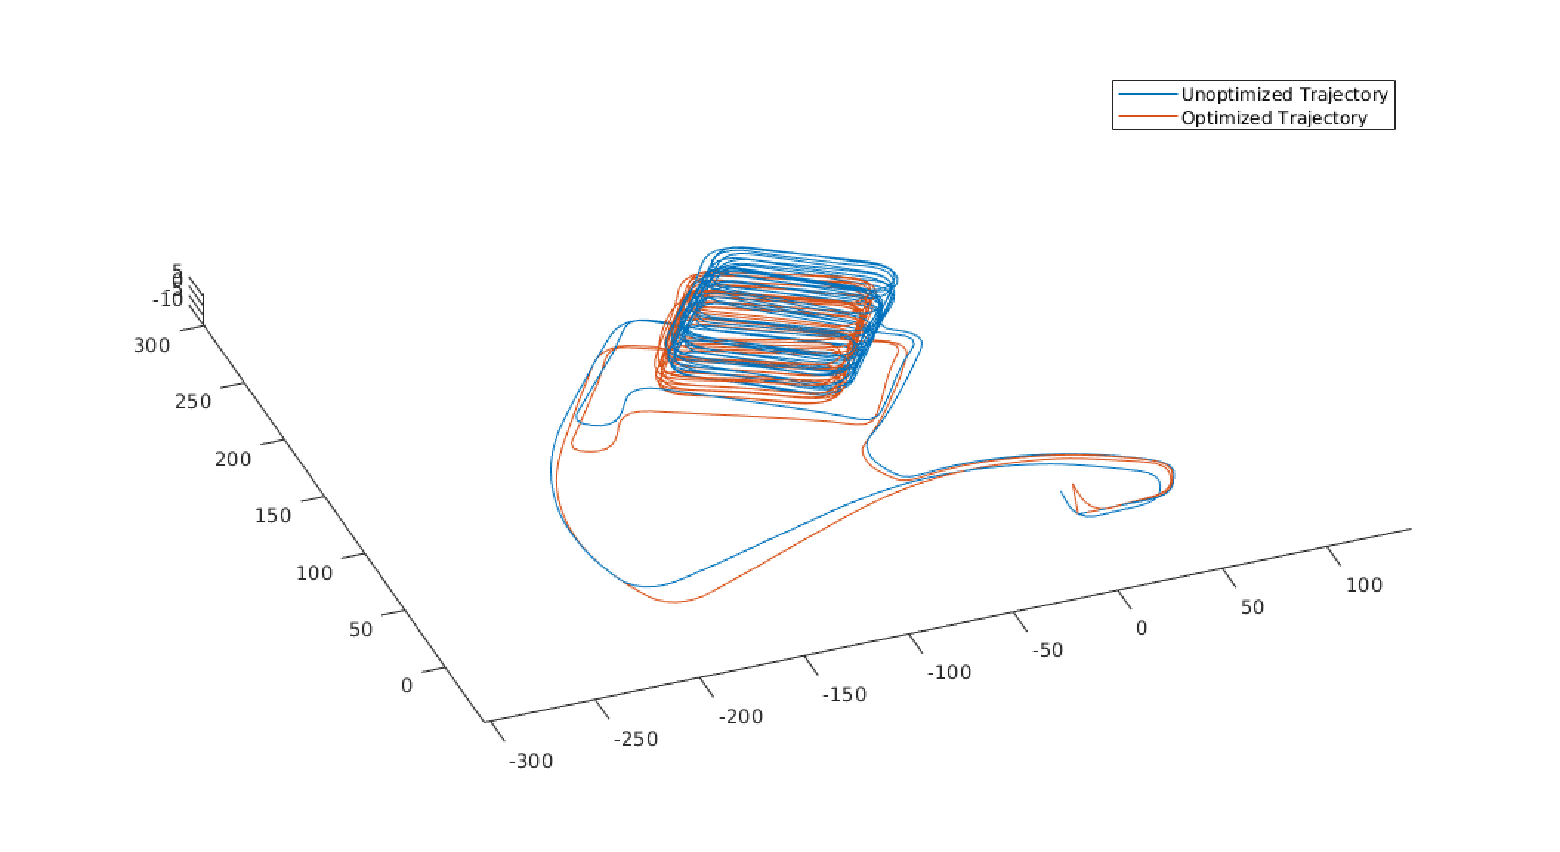
\includegraphics[width=0.8\textwidth]{result_task_2c.png}
    \caption{Expected result for task 2 C.}
    \label{fig:task2c}
\end{figure}

\end{document}